% \section{Experiments}
\section{实验}

\begin{figure*}[t!]
  \centering
  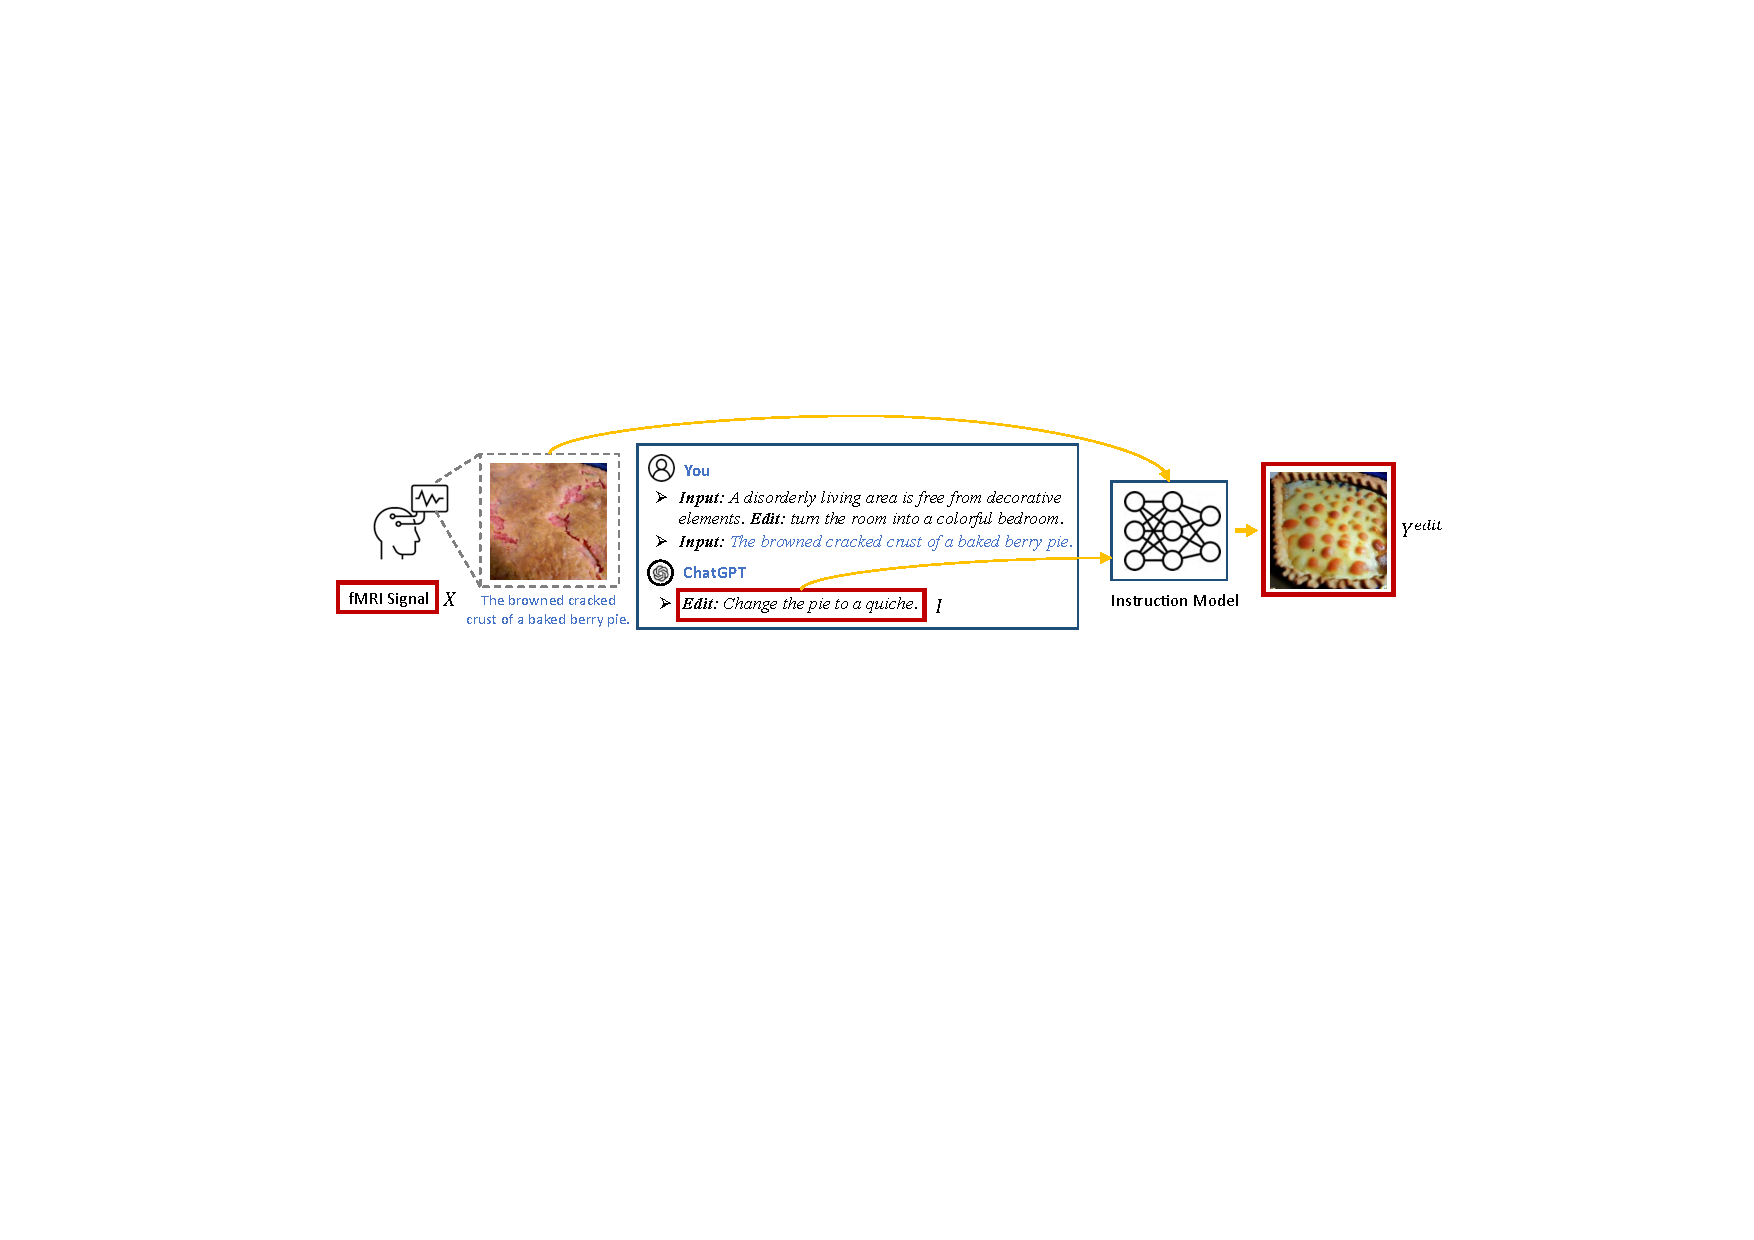
\includegraphics[width=.98\linewidth]{figs/data_pipeline2.pdf}
%   \caption{\textbf{Illustration of Dataset Pipeline.}
%   Given the paired fMRI signal $X$ and its corresponding visual stimuli $Y$ in NSD~\cite{allen2022massive}, we first query LLMs with image caption to obtain possible instruction $I$. Then the instruction, coupled with visual stimuli, is utilized prompt a visual instruction model for manipulated image $Y^{edit}$.
%   Finally, the triplets of $(X, I, Y^{edit})$, are constructed (red boxes).
%   }
  \caption{\textbf{数据集流水线图解。}
  给定 NSD 数据集~\cite{allen2022massive} 中成对的 fMRI 信号 $X$ 及其对应的视觉刺激 $Y$，我们首先利用图像描述查询大语言模型（LLM），以获取可能的指令 $I$。然后，将该指令与视觉刺激结合，用于提示视觉指令模型生成被操纵的图像 $Y^{edit}$。最后，构建出 $(X, I, Y^{edit})$ 三元组（如红框所示）。
  }
  \label{fig:data_pipeline}
\end{figure*}

% \textbf{Datasets.} To validate our proposed approach, we leverage the NSD~\cite{allen2022massive} dataset, the largest neuro-imaging dataset containing densely sampled fMRI data.
\textbf{数据集。} 为了验证我们提出的方法，我们采用了 NSD~\cite{allen2022massive} 数据集，这是目前包含密集采样 fMRI 数据的最大神经成像数据集。
% Participants are asked to view 9000-10000 different pictures over 30-40 MRI scanning sessions.
参与者被要求在 30 到 40 次 MRI 扫描阶段内观看 9000 到 10000 张不同的图片。
% These images are extracted from COCO dataset~\cite{lin2014microsoft}, and corresponding captions are also available. In our experiments, we choose subject 1 from NSD.
这些图像提取自 COCO 数据集~\cite{lin2014microsoft}，并附有相应的描述文本。在我们的实验中，我们选择了 NSD 数据集中的受试者 1（subject 1）。
% For each subject, a total of 9841 image stimuli are presented, with 982 images set aside for validation.
对于每位受试者，共呈现 9841 张图像刺激，其中 982 张图像被留作验证集。
% In our setting, we require triplets of fMRI data, instructions and edited images to train and evaluate our model.
在我们的设定中，我们需要由 fMRI 数据、指令和编辑后图像组成的三元组来训练和评估我们的模型。
% Since such a dataset does not exist, we augment the NSD dataset using Large Language Models (LLMs), as illustrated in Fig.~\ref{fig:data_pipeline}. Specifically, LLMs generate instructions, while a pre-trained visual instruction model accounts for obtaining corresponding edited image.
由于目前不存在这样的数据集，我们利用大语言模型（LLM）对 NSD 数据集进行了扩充，如图~\ref{fig:data_pipeline} 所示。具体而言，LLM 生成指令，而预训练的视觉指令模型负责获取相应的编辑后图像。
% For easy access, we utilize text-davinci-003 engine of ChatGPT~\cite{brown2020language} for in-context instruction synthesis and instructDiffusion~\cite{geng2023instructdiffusion} for visual instruction. Replacing these with more advanced models such as GPT-4V(ison)~\cite{openai2023gpt} or DALL·E 3~\cite{openai2023dalle3} could further improve the dataset quality.
为便于实现，我们利用 ChatGPT~\cite{brown2020language} 的 text-davinci-003 引擎进行上下文指令合成，并使用 instructDiffusion~\cite{geng2023instructdiffusion} 进行视觉指令操作。将这些模型替换为更先进的模型（如 GPT-4V(ision)~\cite{openai2023gpt} 或 DALL·E 3~\cite{openai2023dalle3}）有望进一步提高数据集的质量。

% \paragraph{Implementation. } During the training stage, we freeze the UNet backbones of both the first and second streams to fully leverage the visual priors pre-trained. The overall training process is divided into two stages.
\paragraph{实现细节。} 在训练阶段，我们冻结了第一流和第二流的 UNet 骨干网络，以充分利用预训练的视觉先验。整个训练过程分为两个阶段。
% In the first stage, we target to translate fMRI signal into the visual domain by regressing the intermediate features of CLIP vision/text embedding. The architecture of the regression network and the training paradigms follow protocols similar to MindEye~\cite{scotti2023reconstructing}.
在第一阶段，我们的目标是通过回归 CLIP 视觉/文本嵌入的中间特征，将 fMRI 信号转换到视觉领域。回归网络的架构和训练范式遵循与 MindEye~\cite{scotti2023reconstructing} 相似的协议。
% Once the parameters of this stream have been trained, they are frozen. The adaptor that bridges two streams is finetuned using our extended synthesized dataset.        
一旦该流的参数训练完毕，它们将被冻结。连接这两个流的适配器则使用我们扩展合成的数据集进行微调。
% We employ the Mean Squared Error (MSE) Loss~\cite{ho2020denoising} typical in diffusion models as our optimization objective.
我们采用扩散模型中典型的均方误差（MSE）损失~\cite{ho2020denoising}作为优化目标。
% Since each image stimulus includes three trials, a total of 24980 trials and 8859 visual stimuli are involved in the training set. For fMRI data with multiple trials, we average their responses for consistency.
由于每个图像刺激包含三次试验（trials），训练集中共涉及 24980 次试验和 8859 个视觉刺激。对于包含多次试验的 fMRI 数据，我们对其响应取平均值以保持一致性。
% For our framework and all the compared models, we set the classifier-free scale to 7.5 for image instruction.
对于我们的框架及所有对比模型，在进行图像指令操作时，我们将无分类器引导尺度（classifier-free scale）设置为 7.5。
% Our models are implemented in PyTorch~\cite{paszke2019pytorch} and trained using 80G Tesla A100 GPUs.
我们的模型在 PyTorch~\cite{paszke2019pytorch} 中实现，并使用 80G 的 Tesla A100 GPU 进行训练。

% \paragraph{Comparisons.} Although our framework is designed for fMRI signal instruction, it also supports basic function of reconstruction. Therefore, we validate our method from both the reconstruction and the instruction perspectives.
\paragraph{对比方法。} 尽管我们的框架是为 fMRI 信号指令而设计的，但它也支持基本的重建功能。因此，我们从重建和指令两个视角对我们的方法进行验证。
% For image reconstruction, we compare our method with the best models currently available that support fMRI-based image reconstruction: Takagi \emph{et.al.}~\cite{takagi2023high}, UniBrain~\cite{mai2023unibrain}, Brain-Diffuser~\cite{ozcelik2023brain} and MindEye~\cite{scotti2023reconstructing}.
在图像重建方面，我们将我们的方法与目前支持基于 fMRI 图像重建的最佳模型进行了比较：Takagi \emph{et.al.}~\cite{takagi2023high}、UniBrain~\cite{mai2023unibrain}、Brain-Diffuser~\cite{ozcelik2023brain} 和 MindEye~\cite{scotti2023reconstructing}。
% Takagi \emph{et.al.}~\cite{takagi2023high} pioneered the utilization of image priors from Stable Diffusion (SD)~\cite{esser2021taming} for fMRI-based image reconstruction.
Takagi \emph{et.al.}~\cite{takagi2023high} 开创了利用稳定扩散（SD）~\cite{esser2021taming}图像先验进行基于 fMRI 图像重建的先河。
% UniBrain~\cite{mai2023unibrain} demonstrates the capability to translate fMRI signals to both image captions and images simultaneously.
UniBrain~\cite{mai2023unibrain} 展示了将 fMRI 信号同时转换为图像描述和图像的能力。
% Brain-Diffuser~\cite{ozcelik2023brain} and MindEye~\cite{scotti2023reconstructing} showcase the effectiveness of mapping to CLIP space in the VersatileDiffusion~\cite{xu2023versatile} setting.
Brain-Diffuser~\cite{ozcelik2023brain} 和 MindEye~\cite{scotti2023reconstructing} 展示了在 VersatileDiffusion~\cite{xu2023versatile} 设定下映射到 CLIP 空间的有效性。
% For instruction, we compare our method with state-of-the-art image manipulation approaches, including SDEdit~\cite{meng2021sdedit}, InstructPix2Pix~\cite{brooks2023instructpix2pix}, InstructDiffusion~\cite{geng2023instructdiffusion} and MagicBrush~\cite{zhang2024magicbrush}.
在指令方面，我们将我们的方法与最先进的图像操纵方法进行了比较，包括 SDEdit~\cite{meng2021sdedit}、InstructPix2Pix~\cite{brooks2023instructpix2pix}、InstructDiffusion~\cite{geng2023instructdiffusion} 和 MagicBrush~\cite{zhang2024magicbrush}。
% SDEdit~\cite{meng2021sdedit} proposes to edit image with Stochastic Differential Equation (SDE).
SDEdit~\cite{meng2021sdedit} 提出利用随机微分方程（SDE）来编辑图像。
% InstructPix2Pix~\cite{brooks2023instructpix2pix} directly trains a Stable Diffusion model conditioned on instructions. InstructDiffusion~\cite{geng2023instructdiffusion} and MagicBrush~\cite{zhang2024magicbrush} further extend the dataset and improve the model performance for instruction-based image editing.
InstructPix2Pix~\cite{brooks2023instructpix2pix} 直接训练了一个以指令为条件的稳定扩散模型。InstructDiffusion~\cite{geng2023instructdiffusion} 和 MagicBrush~\cite{zhang2024magicbrush} 进一步扩展了数据集，并提升了模型在基于指令的图像编辑方面的性能。

% \subsection{Quantitative Evaluation}
\subsection{定量评估}

\begin{table*}[t]
\setlength{\tabcolsep}{9pt}
\renewcommand{\arraystretch}{1.1}
\centering
% \caption{\textbf{Quantitative results of image reconstruction on the Natural Scenes Dataset (NSD)~\cite{allen2022massive}.}}
\caption{\textbf{自然场景数据集（NSD）~\cite{allen2022massive}上的图像重建定量结果。}}
\label{table:rec}
\begin{tabular}{lcccccccc}
\toprule
 & \multicolumn{4}{c}{Low-Level Metrics} & \multicolumn{4}{c}{High-Level Metrics} \\
\cmidrule(lr){2-5} \cmidrule(lr){6-9}
Method & PixCorr $\uparrow$ & SSIM $\uparrow$ & Alex(2) $\uparrow$ & Alex(5) $\uparrow$ & Incep $\uparrow$ & CLIP $\uparrow$ & Eff $\downarrow$ & SwAV $\downarrow$ \\
\midrule
Takagi \emph{et.al.}~\cite{takagi2023high} & - & - & 0.830 & 0.830 & 0.760 & 0.770 & - & - \\
UniBrain~\cite{mai2023unibrain} & 0.249 & \underline{0.330} & 0.929 & 0.956 & 0.878 & 0.923 & 0.766 & 0.407 \\
Brain-Diffuser~\cite{ozcelik2023brain} & 0.254 & \textbf{0.356} & 0.942 & 0.962 & 0.872 & 0.915 & 0.775 & 0.423 \\
MindEye~\cite{scotti2023reconstructing} & \underline{0.309} & 0.323 & \underline{0.947} & \underline{0.978} & \underline{0.938} & \textbf{0.941} & \textbf{0.645} & \underline{0.367} \\
\hline
\rowcolor{mygrey} \textbf{\model{}} & \textbf{0.327} &  0.315 & \textbf{0.951} & \textbf{0.978} & \textbf{0.939} & \underline{0.934} & \underline{0.653} & \textbf{0.360} \\
\bottomrule
\end{tabular}
\end{table*}



\begin{table*}[t]
\setlength{\tabcolsep}{11pt}
\renewcommand{\arraystretch}{1.1}
\centering
% \caption{\textbf{Quantitative results of image instruction on the Natural Scenes Dataset (NSD)~\cite{allen2022massive}.}}
\caption{\textbf{自然场景数据集（NSD）~\cite{allen2022massive}上的图像指令定量结果。}}
\label{table:edit}
\begin{tabular}{lccccc}
\toprule
Method & InstructPix2Pix~\cite{brooks2023instructpix2pix} & InstructDiff~\cite{geng2023instructdiffusion} & MagicBrush~\cite{zhang2024magicbrush} & SDEdit~\cite{meng2021sdedit} & \textbf{\model{}} \\
\midrule
\textbf{CLIP-I} & \textbf{0.664} & 0.643 & 0.649 & 0.577 & \cellcolor{mygrey} \underline{0.657} \\
\textbf{DiNO-I} & \textbf{0.305} & 0.274 & 0.289 & 0.181 & \cellcolor{mygrey} \underline{0.301} \\
\textbf{CLIP-D} & 0.090 & \underline{0.113} & 0.105 & 0.101 & \cellcolor{mygrey} \textbf{0.114} \\
\bottomrule
\end{tabular}
\end{table*}

\begin{table*}[t!]
\setlength{\tabcolsep}{22pt}
\renewcommand{\arraystretch}{1.1}
\centering
% \caption{\textbf{The ablation over model design on Natural Scenes Dataset (NSD)~\cite{allen2022massive}.}}
\caption{\textbf{自然场景数据集（NSD）~\cite{allen2022massive}上针对模型设计的消融实验。}}
\label{table:ablation}
\begin{tabular}{lcccc}
\toprule
Method & wo / Asynch & wo / Adaptor Injection & wo / LLMs & \textbf{Full Model} \\
\midrule
\textbf{CLIP-I} & 0.639 & 0.600 & 0.650 & \cellcolor{mygrey} \textbf{0.657} \\
\textbf{Dino-I} & 0.299 & 0.184 & 0.292 & \cellcolor{mygrey} \underline{0.301} \\
\textbf{CLIP-D} & 0.112 & \textbf{0.135} & 0.118 & \cellcolor{mygrey} 0.114 \\
\bottomrule
\end{tabular}
\end{table*}

% \textbf{Evaluation Metric.}  For image reconstruction, we use both low-level and high-level metrics to measure the semantic correctness of our results.
\textbf{评估指标。} 在图像重建方面，我们同时使用低级（low-level）和高级（high-level）指标来衡量结果的语义正确性。
% Specifically, we choose \textbf{PixCorr}, \textbf{SSIM}, \textbf{Alex(2)} and \textbf{Alex(5)} for low-level measurements while \textbf{Incep}, \textbf{CLIP}, \textbf{Eff} and \textbf{SwAV} are utilized for high-level semantic evaluation, following the evaluation protocol of MindEye~\cite{scotti2023reconstructing}.
具体而言，我们选择 \textbf{PixCorr}、\textbf{SSIM}、\textbf{Alex(2)} 和 \textbf{Alex(5)} 作为低级指标测量，而利用 \textbf{Incep}、\textbf{CLIP}、\textbf{Eff} 和 \textbf{SwAV} 进行高级语义评估，这遵循了 MindEye~\cite{scotti2023reconstructing} 的评估协议。
% For instruction-based evaluation, we use CLIP~\cite{radford2021learning} image similarity (\textbf{CLIP-I}) and Dino-V2~\cite{oquab2023dinov2} image similarity (\textbf{Dino-I}) to measure the cosine similarity between edited and original images.
对于基于指令的评估，我们使用 CLIP~\cite{radford2021learning} 图像相似度（\textbf{CLIP-I}）和 Dino-V2~\cite{oquab2023dinov2} 图像相似度（\textbf{Dino-I}）来测量编辑后图像与原始图像之间的余弦相似度。
% Additionally, we use CLIP text-image direction similarity~\cite{gal2022stylegan} (\textbf{CLIP-D}) evaluates how changes in images correspond to changes in their captions.
此外，我们使用 CLIP 文本-图像方向相似度~\cite{gal2022stylegan}（\textbf{CLIP-D}）来评估图像的变化与描述文本变化之间的对应关系。

% \paragraph{Evaluation Results.} The comparison results for image reconstruction from fMRI signals are presented in Table~\ref{table:rec}. Our results exhibit superior performance in low-level semantic consistency and competitive results in high-level metrics.
\paragraph{评估结果。} 基于 fMRI 信号进行图像重建的对比结果展示在表~\ref{table:rec} 中。我们的结果在低级语义一致性上表现出优越的性能，在高级指标上也取得了极具竞争力的结果。
% One possible reason for this is the mixed mapping strategy in the first stream, where we regress both CLIP visual and text embeddings via latent diffusion. We speculate that this practice helps strike a balance between low- and high-level semantic formation.
导致这一结果的一个可能原因在于第一流中的混合映射策略，我们在该流中通过潜在扩散同时回归 CLIP 视觉和文本嵌入。我们推测，这种做法有助于在低级和高级语义形成之间取得平衡。
% Notably, although our framework is not specifically designed for the reconstruction task, it achieves performance comparable to specialized approaches.
值得注意的是，尽管我们的框架并非专门为重建任务设计，但它实现了与专门方法相媲美的性能。

% For image instruction performance, we present the comparison results in Table~\ref{table:edit}. Our method achieves superior results in Dino-V2 image similarity and CLIP text-image direction (CLIP-D) similarity, demonstrating its capability to manipulate visual imagery underlying fMRI signals aligned with human instruction.
关于图像指令性能，我们在表~\ref{table:edit} 中展示了对比结果。我们的方法在 Dino-V2 图像相似度和 CLIP 文本-图像方向（CLIP-D）相似度方面取得了优越的结果，证明了其根据人类指令操纵 fMRI 信号底层的视觉意象的能力。
% However, in the CLIP image similarity metric, our approach scores lower than InstructPix2Pix~\cite{brooks2023instructpix2pix} because they tend towards under-editing, making minimal changes to the input images. Consequently, their results show inferior performance in terms of the CLIP-D metric.
然而，在 CLIP 图像相似度指标上，我们方法的得分低于 InstructPix2Pix~\cite{brooks2023instructpix2pix}，这是因为后者倾向于欠编辑（under-editing），仅对输入图像做出了极小的更改。因此，它们的结果在 CLIP-D 指标上表现不佳。

% \subsection{Qualitative Evaluation}
\subsection{定性评估}
\begin{figure*}[t!]
  \centering
  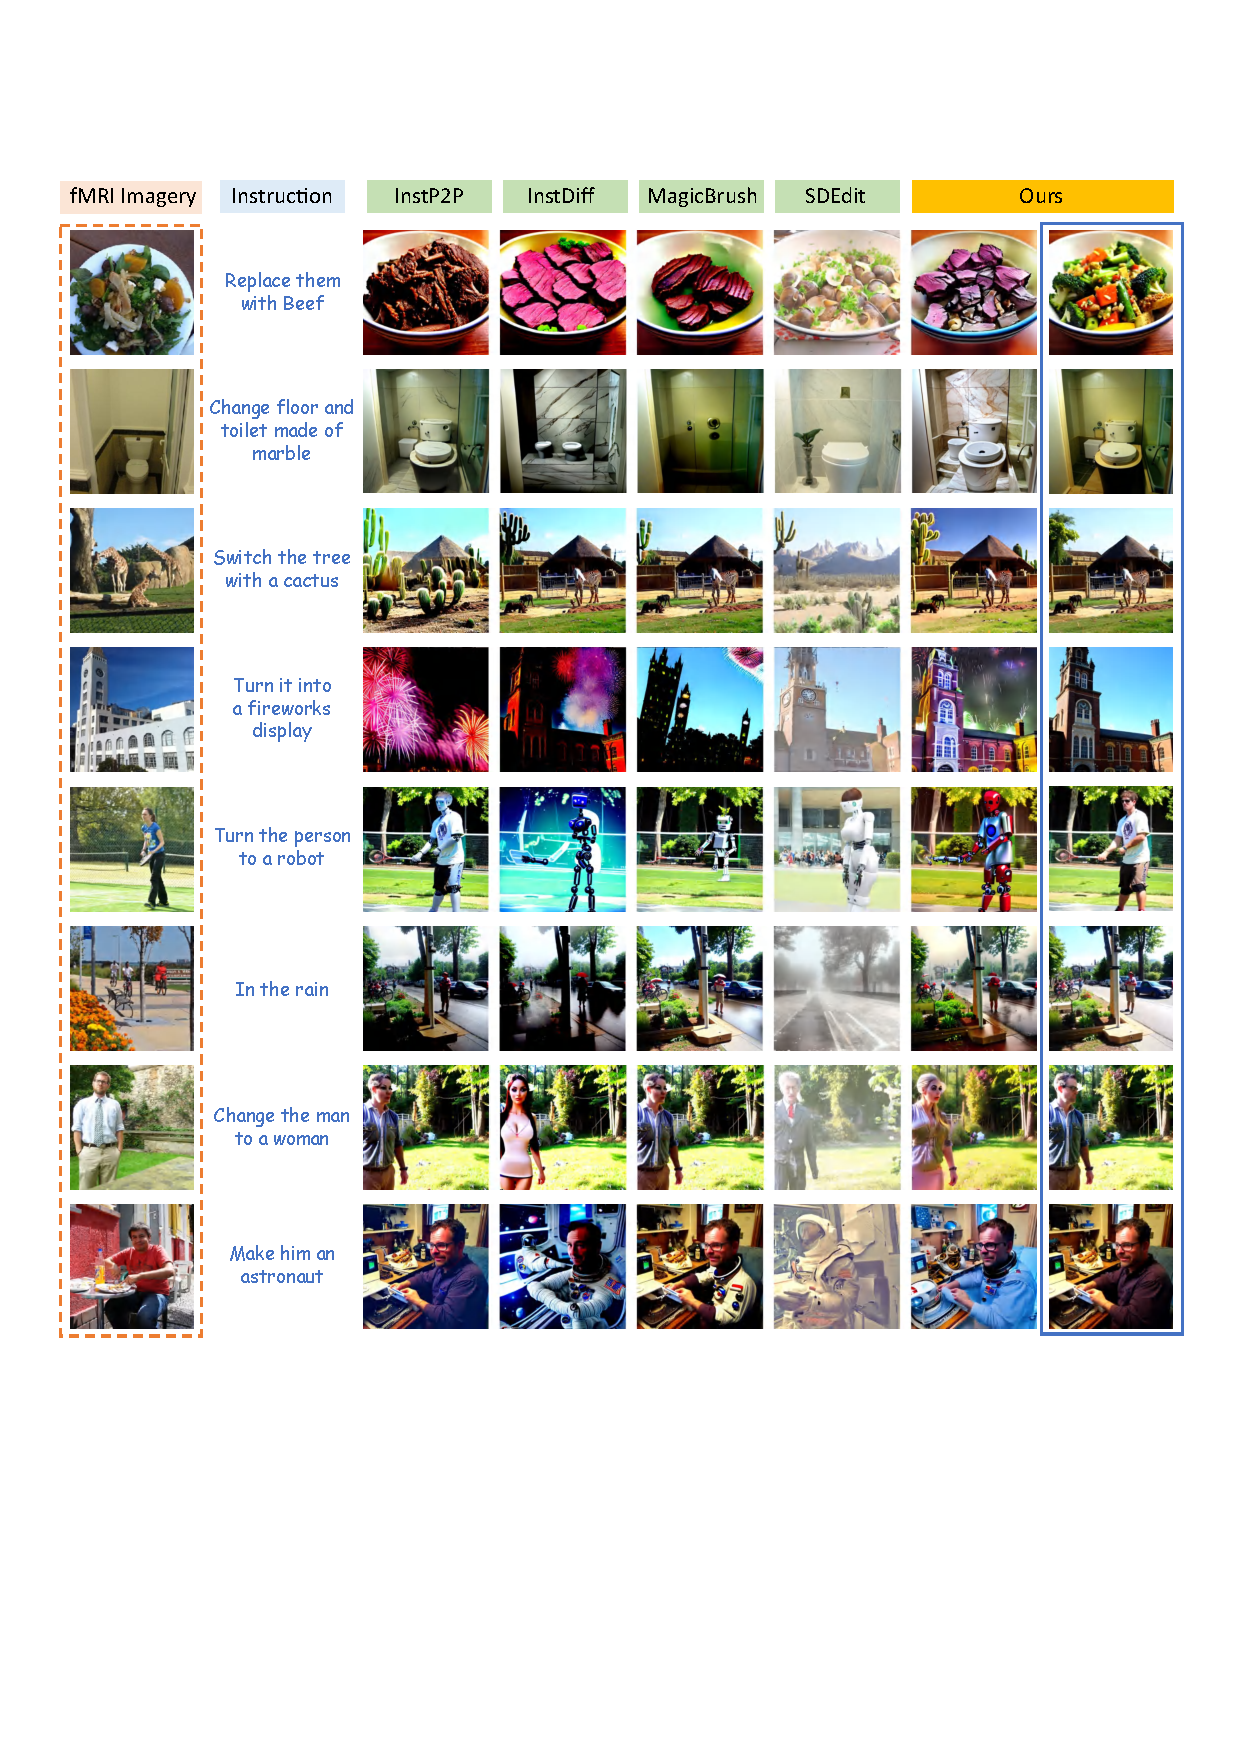
\includegraphics[width=\linewidth]{figs/qual1.pdf}
%   \caption{\textbf{Qualitative Comparison.} In the first column list the visual stimulus of fMRI signal while the last column demonstrates input images used by other approaches. InstP2P~\cite{brooks2023instructpix2pix} struggles on capturing instruction intention (see last 4 rows). InstDiff~\cite{geng2023instructdiffusion} and MagicBrush~\cite{zhang2024magicbrush} tends to over-edit irrelevant regions (see toilet). SDEdit~\cite{meng2021sdedit} suffers from inferior image quality. Our method well balances the content preservation and instruction conformation.
%   }
  \caption{\textbf{定性比较。} 第一列列出了 fMRI 信号的视觉刺激，而最后一列展示了其他方法所使用的输入图像。InstP2P~\cite{brooks2023instructpix2pix} 难以捕捉指令意图（见最后 4 行）。InstDiff~\cite{geng2023instructdiffusion} 和 MagicBrush~\cite{zhang2024magicbrush} 倾向于过度编辑无关区域（见马桶示例）。SDEdit~\cite{meng2021sdedit} 则面临图像质量较低的问题。我们的方法在内容保留与遵循指令之间取得了良好的平衡。
  }
  \label{fig:qual}
\end{figure*}

% \textbf{Image Generation Paradigm.} Since there are no similar studies supporting the direct instruction of fMRI signals, we adapt state-of-the-art image manipulation methods to evaluate the instruction capability of our model.
\textbf{图像生成范式。} 由于目前没有支持直接对 fMRI 信号发出指令的类似研究，我们将最先进的图像操纵方法进行了适配，以评估我们模型的指令能力。
% Specifically, we first generate fMRI instructions using our approach. We then use the obtained intermediate reconstruction $Y^{Rec}$, along with the instruction text, as input to these methods for editing.
具体而言，我们首先使用我们的方法生成 fMRI 指令结果。然后，我们将获取的中间重建图像 $Y^{Rec}$ 与指令文本一起作为输入，提供给这些方法进行编辑。

% \paragraph{Evaluation Results.} We demonstrate the qualitative evaluation results in Figure~\ref{fig:qual}.
\paragraph{评估结果。} 我们在图~\ref{fig:qual} 中展示了定性评估结果。
% We observe that InstructPix2Pix~\cite{brooks2023instructpix2pix} tends to preserve its original content and struggles to follow instructions (see the last 4 rows).
我们观察到 InstructPix2Pix~\cite{brooks2023instructpix2pix} 倾向于保留原始内容，难以遵循指令（见最后 4 行）。
% In contrast, InstructDiffusion~\cite{geng2023instructdiffusion} and MagicBrush~\cite{zhang2024magicbrush} are capable of better following instructions, but often change irrelevant attributes (e.g., the object shape such as the toilet and robot, or the background).
相比之下，InstructDiffusion~\cite{geng2023instructdiffusion} 和 MagicBrush~\cite{zhang2024magicbrush} 能够更好地遵循指令，但常常改变无关的属性（例如，诸如马桶和机器人等物体的形状，或背景）。
% For SDEdit~\cite{meng2021sdedit}, it also faces challenges in preserving unrelated regions and suffers from inferior image quality.
对于 SDEdit~\cite{meng2021sdedit}，它在保留无关区域方面同样面临挑战，并且生成的图像质量较差。
% In contrast, our approach strikes a balance between content preservation and instruction conformation (See the pose of the woman and the cactus shape), which we speculate is attributed to the dual-stream architecture where intermediate features are able to influence instruction progress constantly.
相反，我们的方法在内容保留与遵循指令之间取得了平衡（请见女人的姿势和仙人掌的形状），我们推测这归功于双流架构，其中中间特征能够持续地影响指令进度。
% It is worth noting that these approaches not only rely on our intermediate reconstruction results but also require tedious sequential operations. In contrast, our proposed framework enables direct fMRI signal instruction, streamlining the process.
值得注意的是，这些方法不仅依赖于我们的中间重建结果，还需要繁琐的串行操作。相比之下，我们提出的框架实现了直接对 fMRI 信号进行指令操作，从而精简了整个流程。

% \subsection{Additional Results}
\subsection{附加结果}

\begin{figure*}[t!]
  \centering
  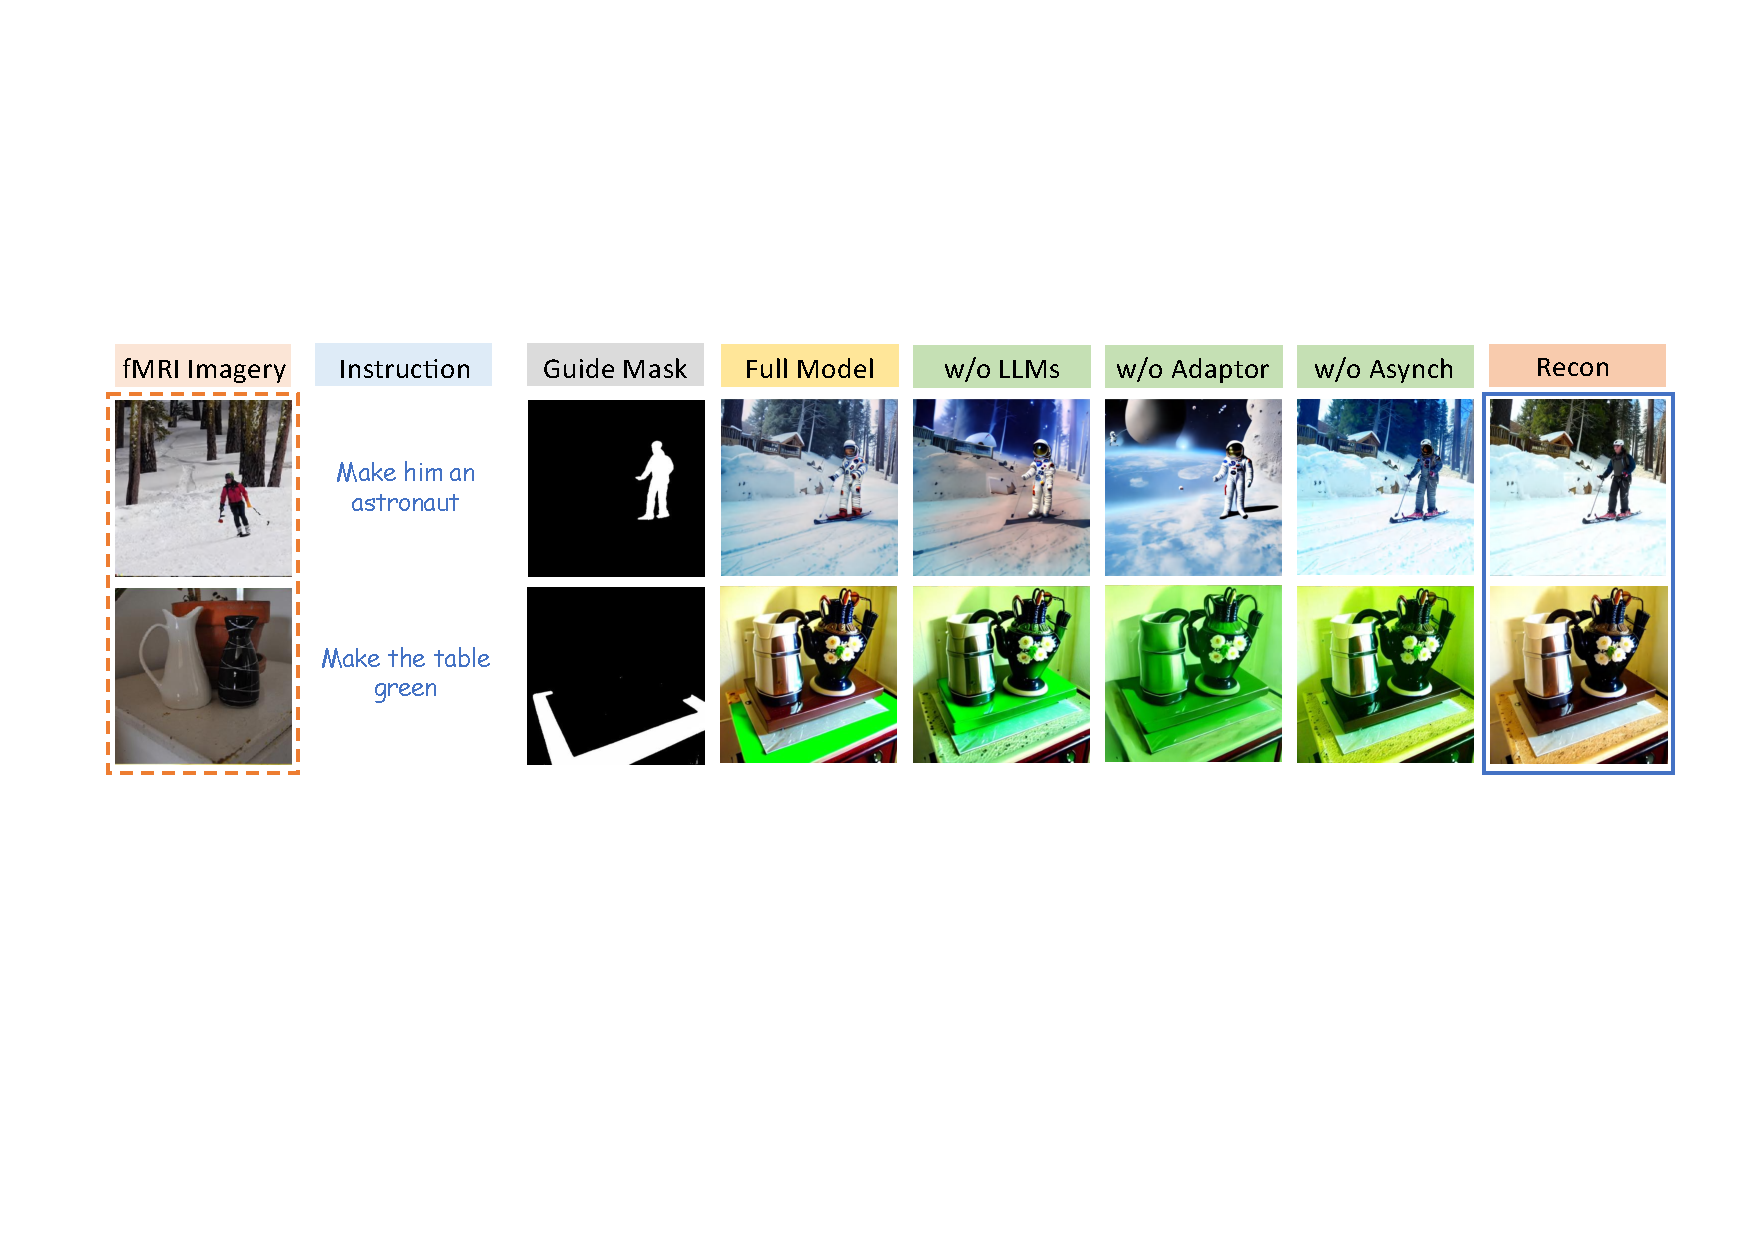
\includegraphics[width=1.0\linewidth]{figs/ablation1.pdf}
%   \caption{\textbf{Ablation Study.} Without feature injection from adaptor, the model struggles on balancing content preservation and instruction conformation. Removing asynchronous strategy brings difficulty on instruction conformation. Through the incorporation of LLMs guided region, our framework is able to precisely operate on relevant spatial locations (see the snow background and table region).
%   }
  \caption{\textbf{消融实验。} 如果没有来自适配器的特征注入，模型在平衡内容保留与遵循指令方面会面临困难。移除异步策略会给遵循指令带来难度。通过引入 LLM 引导的区域，我们的框架能够精确地在相关的空间位置上进行操作（见雪景背景和桌子区域的示例）。
  }
  \label{fig:ablation}
\end{figure*}

% \paragraph{Ablation Study.} We conducted ablation studies focusing on three important aspects of our method: the asynchronous diffusion strategy, the injection of adaptor features, and the use of LLM-guided region-aware attention.
\paragraph{消融实验。} 我们重点针对本方法的三个重要方面进行了消融实验：异步扩散策略、适配器特征的注入以及 LLM 引导的区域感知注意力的使用。
% The experiments were carried out by (1) removing the asynchronous paradigm, (2) eliminating adaptor feature injection, and (3) excluding the LLMs agent. The numerical results are shown in Table~\ref{table:ablation}, and the visualization results are presented in Fig.~\ref{fig:ablation}.
实验通过以下方式进行：(1) 移除异步范式，(2) 取消适配器特征注入，(3) 排除 LLM 代理。数值结果见表~\ref{table:ablation}，可视化结果展示在图~\ref{fig:ablation} 中。
% Eliminating the asynchronous strategy makes it difficult for the instruction flow to comprehend aligned visual content, resulting in inferior performance.
消除异步策略使得指令流难以理解对齐的视觉内容，导致性能下降。
% When adaptor feature injection is removed, the instruction flow lacks sufficient visual information to identify instruction-relevant regions. Consequently, the instruction results deviate from the interpreted visual contents of the first stream, leading to poor performance in terms of both CLIP and Dino image similarity.
当移除适配器特征注入时，指令流缺乏充足的视觉信息来识别与指令相关的区域。因此，指令结果偏离了第一流解释出的视觉内容，导致 CLIP 和 Dino 图像相似度的表现都不佳。
% Without LLMs, the model struggles to perform precise operations within the intended spatial regions.
如果没有 LLM，模型难以在预期的空间区域内执行精确操作。
% The full model effectively strikes a balance between identity preservation and instruction conformation, achieving visually pleasant results.
完整模型有效地在保持身份特征与遵循指令之间取得了平衡，实现了视觉上令人愉悦的结果。

% \paragraph{Multi-Modal Instruction.}
\paragraph{多模态指令。}
\begin{figure*}[t!]
  \centering
  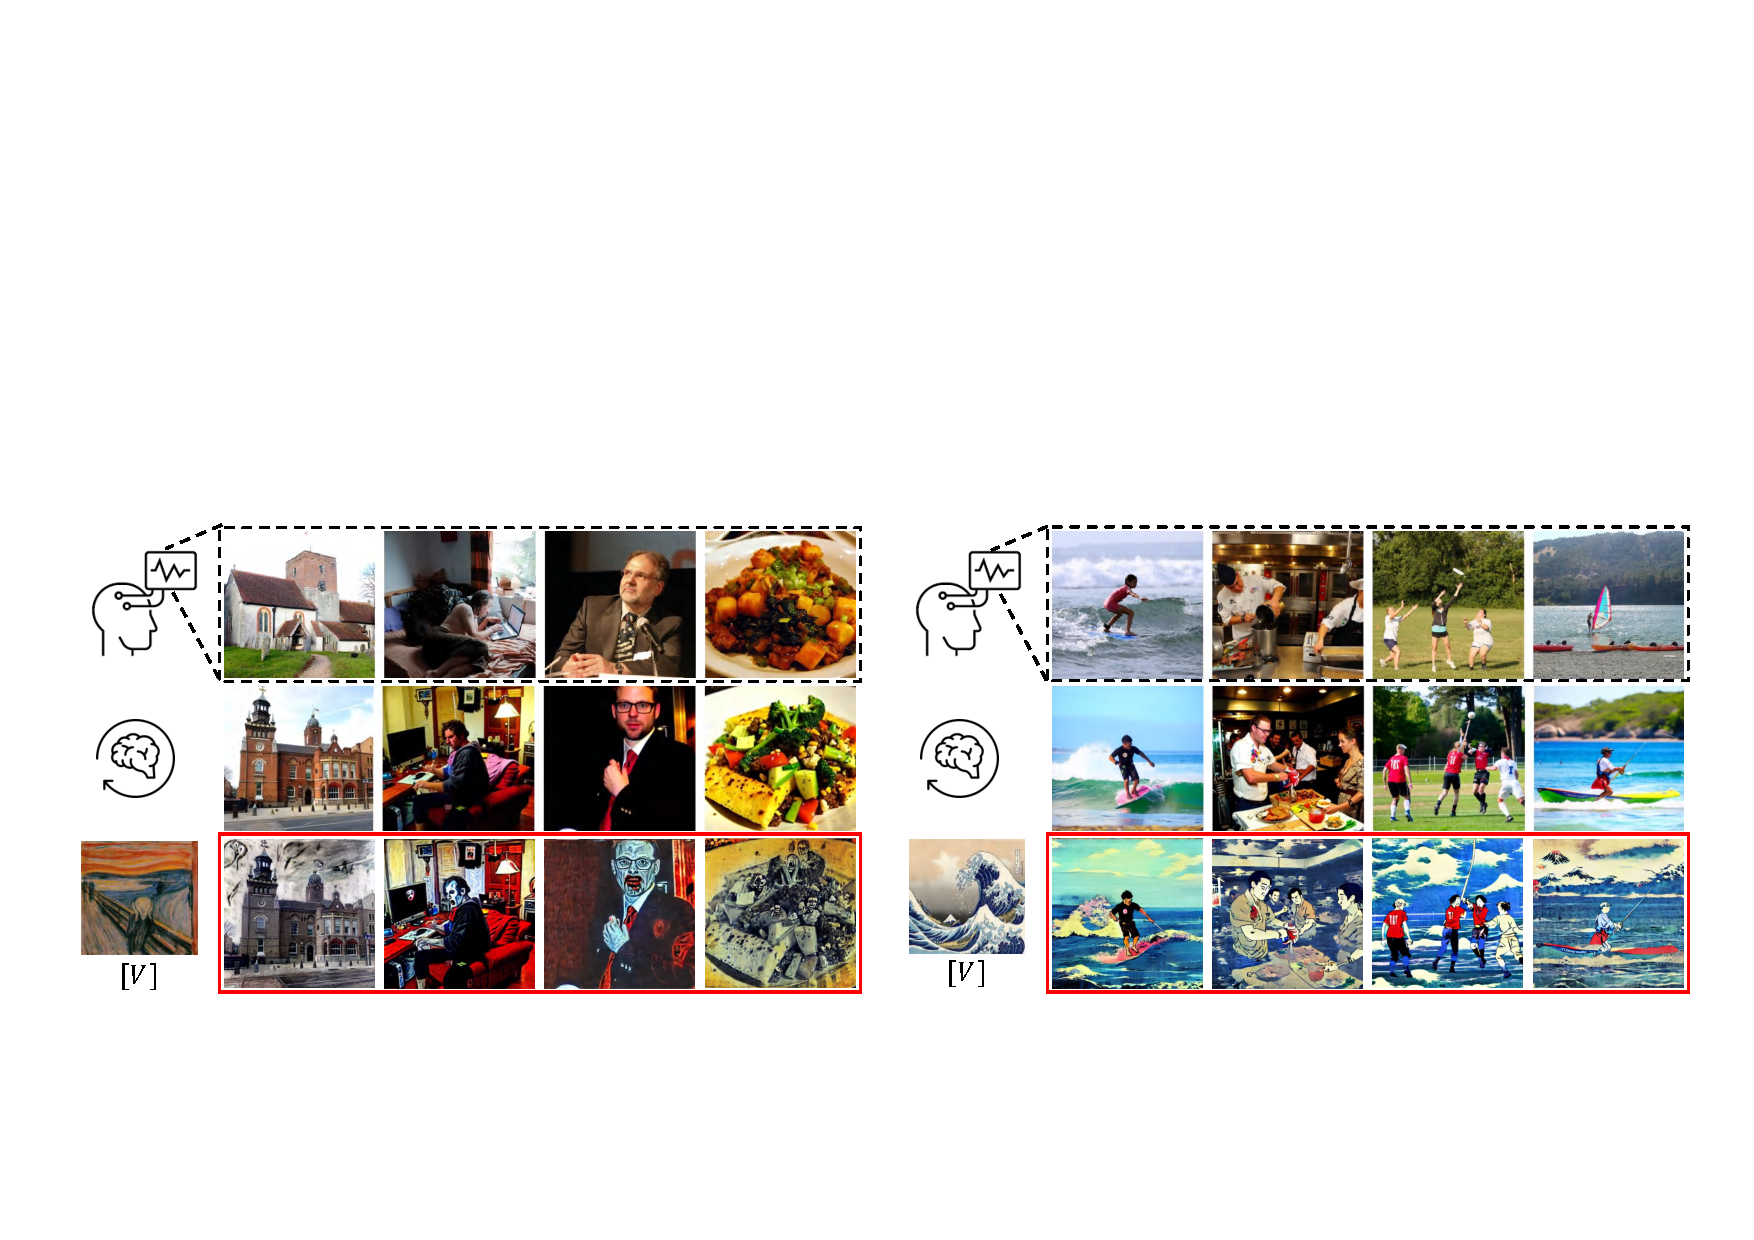
\includegraphics[width=1.0\linewidth]{figs/style.pdf}
%   \caption{\textbf{Demonstration Results of Multi-Modal Instruction.} First row list the visual stimulus while second row depict our intermediate reconstructions. The manipulation results via \emph{In the [V] style} are shown within red boxes of the last row.}
  \caption{\textbf{多模态指令演示结果。} 第一行展示了视觉刺激，第二行描绘了我们的中间重建结果。基于“\emph{以 [V] 风格（In the [V] style）}”的操纵结果显示在最后一行的红框内。}
  \label{fig:style}
\end{figure*}
% Here we showcase the ability of our model to handle multi-modal instruction and achieve style manipulation. With minimal effort, our model can be extended to support visual instruction.
在此，我们展示了模型处理多模态指令并实现风格操纵的能力。只需极少量的修改，我们的模型即可扩展为支持视觉指令。
% Specifically, we modify the instruction description to ``In the [V] style'' where the style ``[V]'' can be obtained using image inversion approaches~\cite{ruiz2023dreambooth,mokady2023null}. It is evident that our approach effectively captures the style of the reference image and applies it to the target.
具体来说，我们将指令描述修改为“以 [V] 风格”，其中风格“[V]”可以使用图像反演方法~\cite{ruiz2023dreambooth,mokady2023null}获得。显而易见，我们的方法有效地捕捉了参考图像的风格并将其应用于目标。